\chapter{Enhedstest}
I dette afsnit beskrives hvordan enhedstest af systemets enheder er udført. Enhedstesten bruges til at verificerer, at hver enkel del virker uafhængigt af andre enheder. 
Der testes primært basal funktionalitet af enhederne, og i nogle tilfælde undersøges hvorvidt krav fra kravspecifikationen opfyldes. I afsnittet testes blandt andet præcision af GPS og højdemåler.

\section{Afstandssensor}

\section{3G}

\newpage
\section{GPS}

Selvom GPSen sidder på 3G/GPS modulet kan det testes for sig selv. 

For at finde den eksakte GPS position fra GPS modulet, testes modulet i forskellige omgivelser. Som kontrol findes koordinaterne for den aktuelle position. Ud fra de fundne koordinater beregnes en afstand i meter, denne afstand fortæller lidt om afvigelsen af GPS modulet. I kravene er der defineret hvor stor en afvigelse GPS modulet må have. Denne afvigelse skal overholdes under tests, men da den aktuelle position har en afvigelse, vil afgivelsen i meter være påvirket. Denne påvirking vil føre til at afvigelsen i meter kan være større end de tilladte 2.5 meter som der er defineret i kravene.
Det har ikke været muligt at teste GPS modulet indendøre, da der ikke var GPS signal tilgængeligt. 

\begin{table}[H]
\begin{tabular}{| p{4cm}| p{4cm}| p{3cm}|}
\hline
GPS moduls koordinater & Aktuelle position & Afvigelse i meter\\\hline
Latitude:10.191518 \newline Longitude: 56.171863 & Latitude: 10.191560 \newline Longitude: 56.171896 & 4 meter\\\hline
Latitude: \newline Longitude & Latitude: \newline Longitude & \\\hline
Latitude: \newline Longitude & Latitude: \newline Longitude & \\\hline

\end{tabular}
\caption{GPS modul}
\label{tab:GPS_modul}
\end{table}



\newpage 
\section{PWM opsætning}

Testen bruges til at fastslå hvorvidt det PWM signal, der genereres af main controller, udsendes med korrekt frekvens og pulsbredde. Testen foregår ved at ændre værdien af compare-registeret\footnote{Se implementation view i \textit{Systemarkitektur og Design}} . Ændringer i compare registerets værdi bør medføre ændringer af pulsbredde i det PWM signal der udsendes fra main controller. 

Indledningsvis indstilles compare-registeret med værdi på 16000, derefter ændres værdien til 24000 og til sidst sættes compare-registerets værdi til 32000. Ved brug af oscilloskop kontrolleres om PWM signal har den korrekte pulsbredde. 

Nedenfor ses en tabel der viser hvordan testen forløb. Efter tabellen vises oscilloskop billeder taget under testen. 

\vspace{0.50cm}

\begin{table}[H]
	\centering
		\begin{tabular}{|c|c|c|c|}
			\hline
			Værdi compare reg. & Frekvens & Forventet pulsbredde & Faktisk pulsbredde \\ \hline
			16000 & 245 Hz & 1.00 ms & 1.00 ms \\ \hline			
			24000 & 245 Hz & 1.50 ms & 1.50 ms \\ \hline
			32000 & 245 Hz & 2.00 ms & 2.00 ms \\ \hline
		\end{tabular}
	\caption{Test resultat}
\end{table}

\vspace{0.50cm}

Figur \ref{fig:PWM_1} vises PWM signal hvor compare register har værdi på 16000. 

\begin{figure}[H]
\centering
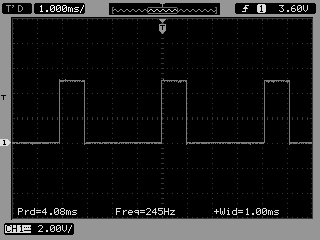
\includegraphics[width=0.7\textwidth]{Billeder/Test/PWM_16000.png}
\vspace{-0.0cm}
\caption{PWM signal - Compare register 16000}
\label{fig:PWM_1}
\end{figure}

\newpage

Figur \ref{fig:PWM_2} vises PWM signal hvor compare register har værdi på 24000. 
\begin{figure}[H]
\centering
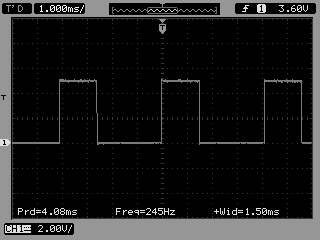
\includegraphics[width=0.7\textwidth]{Billeder/Test/PWM_24000.png}

\caption{PWM signal - Compare register 24000}
\label{fig:PWM_2}
\end{figure}

\vspace{0.5cm}

Figur \ref{fig:PWM_3} vises PWM signal hvor compare register har værdi på 32000. 
\begin{figure}[H]
\centering
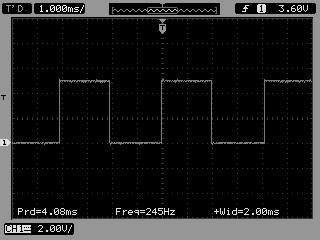
\includegraphics[width=0.7\textwidth]{Billeder/Test/PWM_32000.png}
\vspace{-0.0cm}
\caption{PWM signal - Compare register 32000}
\label{fig:PWM_3}
\end{figure}
